%!TEX root = ../../../adrien_gomar_phd.tex

For an aircraft in steady flight conditions, 
lift balances weight and 
thrust balances drag. This explains why engineers try
indefinitely to reduce weight while increasing
thrust. A trade-off between both aspects is to work
on the propulsive efficiency of the engine. In this
section, general information on propulsion are given,
that leads to the concepts of propeller and
contra-rotating open rotor.

\subsection{Thrust equation}
\label{sub:cror_thrust}

The force applied on an engine, namely the thrust,
comes from the static pressure
distribution and the viscosity of the wetted areas.
To compute it, we assume for simplicity that:
 \begin{itemize} \itemsep0pt \parskip0pt
  \item the engine is schematically represented by a tube,
  as shown in Figure~\ref{fig:engine_parametrization},
  \item the flow is steady (steady-state hypothesis),
  \item the viscosity effects are negligible compared
  to the pressure effects,
  \item the pressure surrounding the engine $p_\infty$
  is constant,
  \item the inlet pressure $p_0$, the outlet pressure
  $p_1$ and the pressure surrounding the engine $p_\infty$ are equal,
  meaning that the nozzle is adapted.
\end{itemize}
The problem parametrization is schematically represented
in Figure~\ref{fig:engine_parametrization}.
\begin{figure}[htp]
  \centering
  \subfigure{
      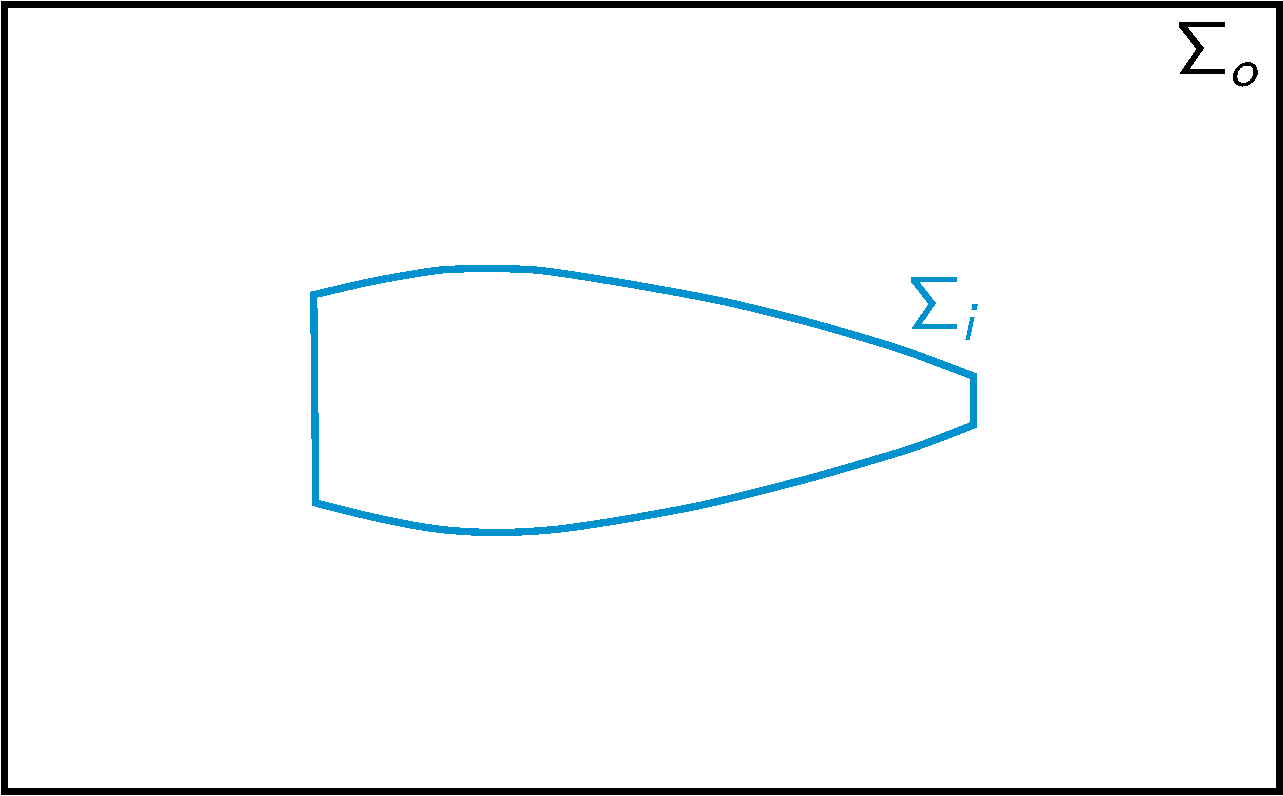
\includegraphics[scale=.3]{control_volume.pdf}}
  \quad\subfigure{
      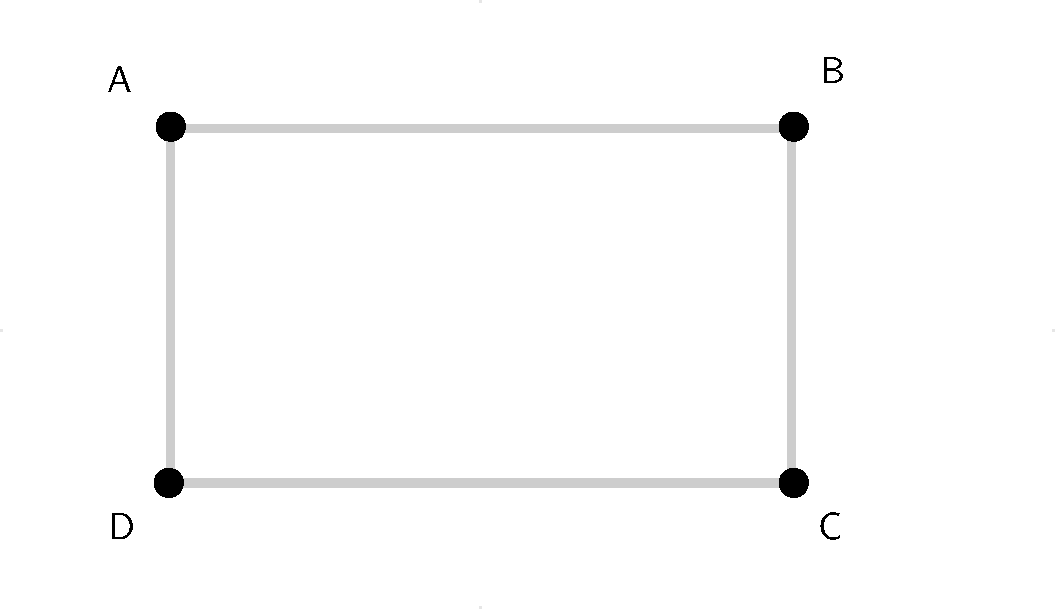
\includegraphics[scale=.3]{control_volume_2.pdf}}
  \caption{Engine parametrization for the computation of the thrust.}
  \label{fig:engine_parametrization}
\end{figure}
With the given hypothesis, the thrust, which is
the resultant force
projected onto the x-axis, is defined as
\begin{equation}
	F_x = \iint_{BC + DA} p_{int} \diff \vec{S} - 
	    \iint_{BC + DA} p_{\infty} \diff \vec{S},
	\label{eq:thrust_1}
\end{equation}
where $p_{int}$ is the internal static
pressure distribution. The integral on
$AB + CD$ is zero due to the projection on
the x-axis.
Moreover, as the surrounding pressure is constant
\begin{equation}
	\iint_{BC + DA} p_{\infty} \diff \vec{S} =
	p_{\infty} \iint_{BC + DA} \diff \vec{S} =
	p_{\infty} (S_{1} - S_{0}).
	\label{eq:thrust_2}
\end{equation}
The distribution of internal pressure is
difficult to estimate. To alleviate this, 
we make use of the Euler’s momentum 
equation applied to the internal fluid
\begin{equation}
	\iint_{S} \left(\rho \vec{V} \cdot \diff \vec{S} \right) V = 
	\iint_{S} p \diff \vec{S}
	\label{eq:thrust_3}
\end{equation}
The velocity being zero at walls, 
the left-hand side of the Eq.~\eqref{eq:thrust_3}
simplifies to
\begin{equation}
	\iint_{S} \left(\rho \vec{V} \cdot \diff \vec{S} \right) V =
	- \rho_0 V_0 S_0 V_0 +  \rho_1 V_1 S_1 V_1 = 
	\dot{m} \left( V_{1} - V_{0} \right),
\end{equation}
where $\dot{m}$ is the mass-flow rate going through the engine.
The right-hand side of Eq.~\eqref{eq:thrust_3}, projected onto
the x-axis, is equal to 
\begin{equation}
	\iint_{S} p \diff \vec{S} = 
	\iint_{BC + DA} p \diff \vec{S} = 
	p_{\infty} \iint_{BC + DA} \diff \vec{S} =
	p_{\infty} (S_{1} - S_{0}),
\end{equation}
since we consider that $p_0 = p_1 = p_\infty$.
Finally the thrust $F_x$ simplifies to
\begin{equation}
	\fbox{$
	F_x = \dot{m} (V_{1} - V_{0})
	$}
	\label{eq:cror_thrust}
\end{equation}
From this simple equation,
one can see that to increase the thrust $F_x$, there are two parameters:
the mass-flow and the axial velocity increment.

\subsection{Global propulsive efficiency}
\label{sub:cror_efficiency}

The global propulsive efficiency $\eta$ measures the 
success in converting a mechanical power into a
propulsive power. It results from the combination
of the kinetic efficiency $\eta_{K}$ and the propulsive efficiency
$\eta_{PR}$
\begin{equation}
	\eta = \eta_{K} \times \eta_{PR}.
\end{equation}
This is schematically represented in Figure~\ref{fig:cror_efficiency}.
\begin{figure}[htp]
  \centering
  \includegraphics*[width=0.5\textwidth]{efficiency.pdf}
  \caption{Efficiency relations from mechanical power to propulsive power.}
  \label{fig:cror_efficiency}
\end{figure}

\paragraph{Kinetic efficiency}
The kinetic efficiency measures the success in converting the mechanical
power $P_m$ into a kinetic power $P_k$
\begin{equation}
	\eta_K = \frac{P_k}{P_m}.
\end{equation}

The mechanical power delivered as input
can be computed through the first thermodynamic principle. In fact, in absence
of heat exchange, the mechanical power $P_m$ can be estimated as
\begin{equation}
	P_m = \dot{m} (h_{i_{1}} - h_{i_{0}}),
\end{equation}
where $h_i$ is the total enthalpy and subscript $0$ and $1$ are
the input and output of the propulsion system, respectively, as represented
in Figure~\ref{fig:engine_parametrization}.
The kinetic power $P_k$ is given by
\begin{equation}
	P_k = \dot{m} \left(\frac{1}{2} V^2_{1} -
	\frac{1}{2} V^2_{0} \right).
\end{equation}
This leads to a kinetic efficiency that can be expressed as
\begin{equation}
	\eta_{K} = \frac{V^2_{1} - V^2_{0}}{2 (h_{i_{1}} - h_{i_{0}})}.
\end{equation}

\paragraph{Propulsive efficiency}
The propulsive efficiency $\eta_{PR}$ measures the success
in creating a propulsive power $P_{pr}$ from a
kinetic power $P_k$
\begin{equation}
	\eta_{PR} = \frac{P_{pr}}{P_k}.
\end{equation}
The propulsive power is computed using the thrust $F_x$
\begin{equation}
	P_{pr} = F_x \times V_{\infty},
\end{equation}
where $V_{\infty}$ is the free-stream velocity.
Finally, if the free-stream velocity is the inlet velocity $V_{0}$
and the inlet and outlet velocities are purely axial
\begin{equation}
	\fbox{$
	\eta_{PR} = \displaystyle \frac{1}{1 + \frac{V_{1} - V_{0}}{2 V_{0}}}
	$}
	\label{eq:cror_propulsive_efficiency}
\end{equation}
This formula means that the most efficient engine produces
a very small velocity increment.

\subsection{Toward propeller engines}
\label{sub:cror_toward_propeller}

One way to improve the environmental footprint of
airplanes engines is to increase the propulsive efficiency
by reducing the kinetic power needed to drive the engine.
According to the propulsive efficiency 
formula, doing so while maintaining the thrust can be achieved through
a higher mass-flow rate. Two new concepts are thus derived from
this simple statement: the
Ultra-High Bypass Ratio (UHBR) which
is basically a turbofan with a larger fan exhaust, and the
propeller, the mass-flow rate of which is not limited
by the architecture, as the blades are not within a nacelle.
In the following section, the propeller engine will be detailed
and the drawbacks of such an architecture will be highlighted to
motivate the use
of a second propeller row, yielding the contra-rotating open rotor
architecture.


